\week{7}{1 Mar.\ 2024}{Sub-Exponential Random Variables}
\section{Sub-exponential distributions}
\begin{problem*}[Exercise 2.7.2]\label{ex2.7.2}
	Prove the equivalence of properties a-d in Proposition 2.7.1 by modifying the proof of Proposition 2.5.2.
\end{problem*}
\begin{answer}
	This is a special case of \hyperref[ex2.7.3]{Exercise 2.7.3}  with \(\alpha = 1\).
\end{answer}

\begin{problem*}[Exercise 2.7.3]\label{ex2.7.3}
	More generally, consider the class of distributions whose tail decay is of the type \(\exp (-ct^\alpha )\) or faster. Here \(\alpha = 2\) corresponds to sub-gaussian distributions, and \(\alpha = 1\), to sub-exponential. State and prove a version of Proposition 2.7.1 for such distributions.
\end{problem*}
\begin{answer}
	The generalized version of Proposition 2.7.1 is known to be the so-called \emph{Sub-Weibull distributions}~\cite{Vladimirova_2020}: Let \(X\) be a random variable. Then the following properties are equivalent; the parameters \(K_i > 0\) appearing in these properties differ from each other by at most an absolute constant factor.
	\begin{enumerate}[(a)]
		\item\label{ex2.7.3:a} The tails of \(X\) satisfy
		      \[
			      \mathbb{P} (\vert X \vert \geq t)
			      \leq 2 \exp (- t^\alpha / K_1) \text{ for all } t \geq 0.
		      \]
		\item\label{ex2.7.3:b} The moments of \(X\) satisfy
		      \[
			      \lVert X \rVert _{L^p}
			      = (\mathbb{E}_{}[\vert X \vert ^p] )^{1 / p}
			      \leq K_2 p^{1 / \alpha } \text{ for all } p \geq 1.
		      \]
		\item\label{ex2.7.3:c} The MGF of \(\vert X \vert \) satisfies
		      \[
			      \mathbb{E}_{}[\exp (\lambda ^\alpha \vert X \vert ^\alpha )]
			      \leq \exp (\lambda ^\alpha K_3^\alpha ) \text{ for all \(\lambda \) such that } 0 \leq \lambda \leq \frac{1}{K_3} .
		      \]
		\item\label{ex2.7.3:d} The MGF of \(\vert X \vert \) is bounded at some point, namely
		      \[
			      \mathbb{E}_{}[\exp (\vert X \vert ^\alpha / K_4^\alpha )] \leq 2.
		      \]
	\end{enumerate}

	\begin{claim}
		\autoref{ex2.7.3:a} \(\implies \) \autoref{ex2.7.3:b}
	\end{claim}
	\begin{explanation}
		Without loss of generality, let \(K_1 = 1\). Then, we have
		\begin{align*}
			\lVert X \rVert _{L^p} ^p
			 & = \int_{0}^{\infty} \mathbb{P} (\vert X \vert ^p \geq t) \,\mathrm{d}t                                           \\
			 & = \int_{0}^{\infty} p u^{p-1} \mathbb{P} (\vert X \vert \geq u) \,\mathrm{d}u \tag*{\(u \coloneqq t^{1 / p}\)}   \\
			 & \leq 2p \int_{0}^{\infty} u^{p-1} e^{-u^\alpha } \,\mathrm{d}u \tag*{from our assumption}                        \\
			 & = \frac{2p}{\alpha } \int_{0}^{\infty} t^{p / \alpha - 1} e^{- t} \,\mathrm{d}t \tag*{\(t \coloneqq u^\alpha \)} \\
			 & = 2 \frac{p}{\alpha } \Gamma (p / \alpha )
			= 2 \Gamma (p / \alpha + 1)
			\lesssim (p / \alpha + 1)^{p / \alpha + 1}
		\end{align*}
		for some constant \(C\) from Stirling's approximation. Hence,
		\[
			\lVert X \rVert _{L^p}
			\lesssim \left( \frac{p}{\alpha } + 1 \right) ^{\frac{1}{\alpha } + \frac{1}{p}}
			= \left( \frac{p}{\alpha } + 1 \right) ^{\frac{1}{\alpha }} \left( \frac{p}{\alpha } + 1 \right)^{\frac{1}{p}}
			\lesssim p^{1 / \alpha }
		\]
		as we desired.
	\end{explanation}

	\begin{claim}
		\autoref{ex2.7.3:b} \(\implies \) \autoref{ex2.7.3:c}
	\end{claim}
	\begin{explanation}
		Firstly, from Taylor's expansion, we have
		\[
			\mathbb{E}_{}[\exp (\lambda ^\alpha \vert X \vert ^\alpha )]
			= 1 + \sum_{k=1}^{\infty} \frac{\lambda ^{\alpha k} \mathbb{E}_{}[\vert X \vert ^{\alpha k}] }{k!}
			\leq 1 + \sum_{k=1}^{\infty} \frac{\lambda ^{\alpha k} \mathbb{E}_{}[\vert X \vert ^{\alpha k}] }{k!}.
		\]
		From \autoref{ex2.7.3:b}, when \(\alpha k \geq 1\), we have \(\mathbb{E}_{}[\vert X \vert ^{\alpha k}] \leq (K_2 (\alpha k)^{1 / \alpha })^{\alpha k} = K_2^{\alpha k} (\alpha k)^k\). On the other hand, for any given \(\alpha > 0\), there are only finitely many \(k \geq 1\) such that \(\alpha k < 1\). Hence, there exists some \(\widetilde{K} _2\) such that
		\[
			\mathbb{E}_{}[\vert X \vert ^{\alpha k}]
			\leq \widetilde{K} _2^{\alpha k} (\alpha k)^k
		\]
		for all \(k \geq 1\). With \(k! \geq (k / e)^k\) from Stirling's approximation, we further have
		\[
			1 + \sum_{k=1}^{\infty} \frac{\lambda ^{\alpha k} \mathbb{E}_{}[\vert X \vert ^{\alpha k}] }{k!}
			\leq 1 + \sum_{k=1}^{\infty} \frac{\lambda ^{\alpha k} \widetilde{K} _2^{\alpha k} (\alpha k)^k }{(k / e)^k}
			= 1 + \sum_{k=1}^{\infty} \lambda ^{\alpha k} \widetilde{K} _2^{\alpha k} (\alpha e)^k
			= 1 + \sum_{k=1}^{\infty} (\widetilde{K} _2^\alpha \lambda ^\alpha \alpha e)^k.
		\]
		Observe that if \(0 < \widetilde{K} _2^\alpha \lambda ^\alpha \alpha e < 1\), we then have
		\[
			\mathbb{E}_{}[\exp (\lambda ^\alpha \vert X \vert ^\alpha )]
			\leq 1 + \sum_{k=1}^{\infty} (\widetilde{K} _2^\alpha \lambda ^\alpha \alpha e)^k
			= \frac{1}{1 - \widetilde{K} _2^\alpha \lambda ^\alpha \alpha e}.
		\]
		As \((1 - x)e^{2x} \geq 1\) for all \(x \in [0, 1 / 2]\), the above is further less than
		\[
			\exp (2 (\widetilde{K} _2 \lambda )^\alpha \alpha e)
			= \exp (\left[ (2 \alpha e)^{1 / \alpha } \widetilde{K} _2 \right] ^\alpha \lambda ^\alpha ).
		\]
		By letting \(K_3 \coloneqq (2 \alpha e)^{1 / \alpha } \widetilde{K} _2\), we have the desired result whenever \(\widetilde{K} _2^\alpha \lambda ^\alpha \alpha e < 1\), or equivalently,
		\[
			0 < \lambda ^\alpha < \frac{1}{\widetilde{K} _2^\alpha \alpha e}
			\iff 0 < \lambda < \frac{1}{\widetilde{K} _2 (\alpha e)^{1 / \alpha }}.
		\]
		Hence, if \(0 < \lambda \leq \frac{1}{\widetilde{K} _2 (2 \alpha e)^{1 / \alpha }} = \frac{1}{K_3}\), the above is satisfied.
	\end{explanation}

	\begin{claim}
		\autoref{ex2.7.3:c} \(\implies \) \autoref{ex2.7.3:d}
	\end{claim}
	\begin{explanation}
		Assuming \autoref{ex2.7.3:c} holds, then \autoref{ex2.7.3:d} is obtained by taking \(\lambda \coloneqq 1 / K_4\) where \(K_4 \coloneqq K_3 (\ln 2)^{-1 / \alpha }\). In this case, \(\lambda = 1 / K_3 \cdot (\ln 2)^{1 / \alpha }\), hence
		\[
			\mathbb{E}_{}[\exp (\lambda ^\alpha \vert X \vert ^\alpha )]
			= \mathbb{E}_{}[\exp (\vert X \vert ^\alpha / K_4^\alpha )]
			\leq \exp (\lambda ^\alpha K_3^\alpha )
		\]
		for all \(0 \leq \lambda = 1 / K_4 \leq 1 / K_3\) from \autoref{ex2.7.3:d} gives
		\[
			\mathbb{E}_{}[\exp (\vert X \vert ^\alpha / K_4 ^\alpha )]
			\leq \exp (\ln 2 \cdot \frac{1}{K_3^\alpha} \cdot K_3^\alpha )
			= 2.
		\]
	\end{explanation}

	\begin{claim}
		\autoref{ex2.7.3:d} \(\implies \) \autoref{ex2.7.3:a}
	\end{claim}
	\begin{explanation}
		Let \(K_4 = 1\) without loss of generality. Then, we have
		\[
			\mathbb{P} (\vert X \vert \geq t)
			= \mathbb{P} (\exp (\vert X \vert ^\alpha ) \geq \exp (t^\alpha ))
			\leq \frac{\mathbb{E}_{}[\exp (\vert X \vert ^\alpha )] }{\exp (t^\alpha )}
			\leq 2 \exp (-t^\alpha ),
		\]
		hence \(K_1 \coloneqq 1\) proves the result.
	\end{explanation}
\end{answer}

\begin{problem*}[Exercise 2.7.4]\label{ex2.7.4}
	Argue that the bound in property c can not be extended for all \(\lambda \) such that \(\lvert \lambda \rvert \leq 1 / K_3\).
\end{problem*}
\begin{answer}
	It's easy to see that in the proof of \hyperref[ex2.7.3]{Exercise 2.7.3}, when we prove \autoref{ex2.7.3:b} \(\implies \) \autoref{ex2.7.3:c}, the condition for \(\lambda \) essentially comes from:
	\begin{itemize}
		\item whether \(1 + \sum_{k=1}^{\infty} (\widetilde{K} _2^\alpha \lambda ^\alpha \alpha e)^k = 1 + \sum_{k=1}^{\infty} (\widetilde{K} _2 \lambda e)^k\) as \(\alpha = 1\) converges; and
		\item the numerical inequality \((1 - x)e^{2x} \geq 1\) for \(x \in [0, 1 / 2]\) such that \(x \coloneqq \widetilde{K} _2 \lambda e\).
	\end{itemize}

	For the first condition, we only need \(\vert \widetilde{K} _2 \lambda e \vert < 1\), hence we don't need positivity for \(\lambda \) at first; however, the second condition indeed requires \(\lambda \geq 0\), and it's impossible to remove as this is tight.

	\begin{center}
		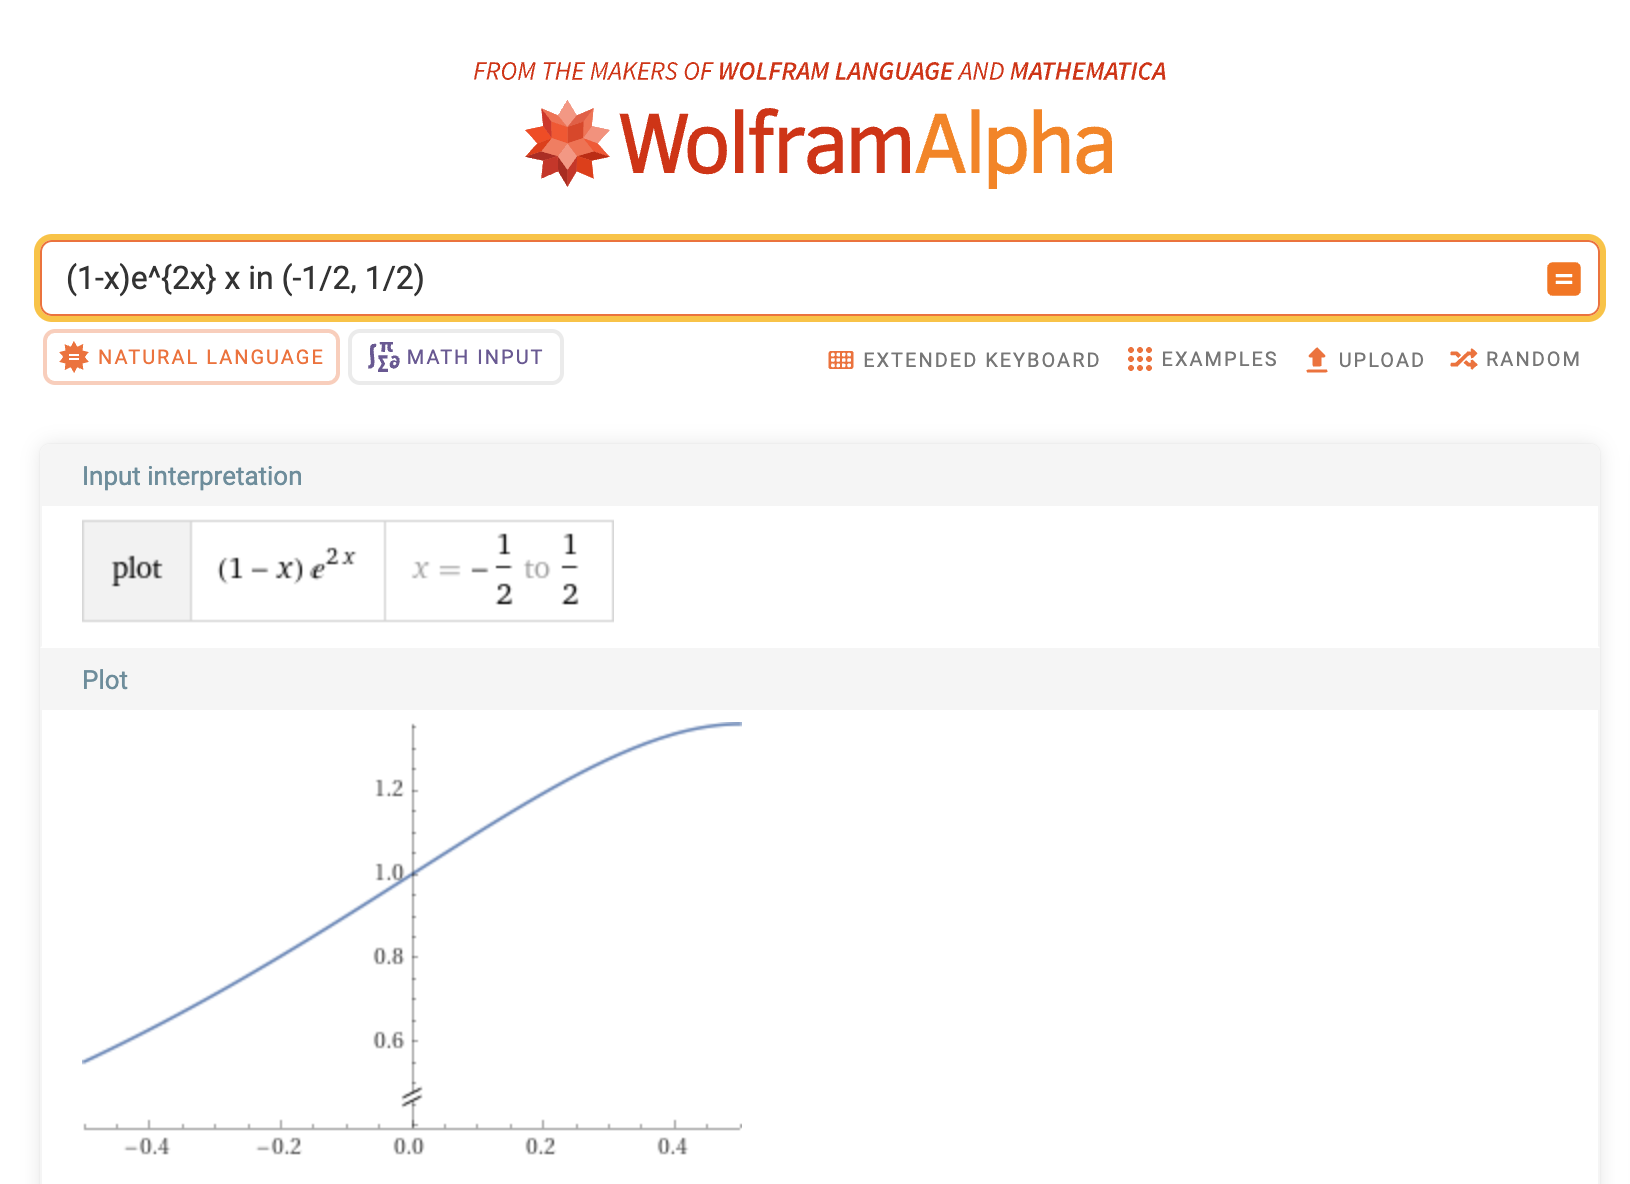
\includegraphics[width=\linewidth]{Figures/ex2.7.4.png}
	\end{center}
\end{answer}

\begin{problem*}[Exercise 2.7.10]\label{ex2.7.10}
	Prove an analog of the Centering Lemma 2.6.8 for sub-exponential random variables \(X\):
	\[
		\lVert X - \mathbb{E}_{}[X] \rVert _{\psi _1}
		\leq C \lVert X \rVert _{\psi _1}.
	\]
\end{problem*}
\begin{answer}
	Since \(\lVert \cdot \rVert _{\psi _2}\) is a norm, we have \(\lVert X - \mathbb{E}_{}[X] \rVert _{\psi _1} \leq \lVert X \rVert _{\psi _1} + \lVert \mathbb{E}_{}[X] \rVert _{\psi _1}\) such that
	\begin{align*}
		\lVert \mathbb{E}_{}[X] \rVert _{\psi _1}
		 & \lesssim \vert \mathbb{E}_{}[X] \vert \tag*{\(\lVert a \rVert _{\psi _1} = \inf _{t > 0} \{ \mathbb{E}_{}[e^{\vert a \vert / t}] \leq 2 \} \lesssim \vert a \vert \)} \\
		 & \leq \mathbb{E}_{}[\vert X \vert ]    \tag*{Jensen's inequality}                                                                                                      \\
		 & = \lVert X \rVert _{L^1}
		\lesssim \lVert X \rVert _{\psi _1}
	\end{align*}
	from Proposition 2.7.1 (b) with \(p = 1\), i.e.,
	\[
		\lVert X \rVert _{L^1} \leq K_{2} \cong \lVert X \rVert _{\psi _1}
	\]
	since \(K_i \cong \lVert X \rVert _{\psi _1} = K_4\).
\end{answer}